\subsection{Developing for Unity}
There were two main aspects to developing for Unity which we rehaul from the sample Unity Haply Gitlab repository:
\subsubsection{Board Configurations}
Since we have differently configured 2DIY Gen 3 Haply boards (and in some cases, Gen 2 boards), we need a way to switch easily between these configurations without spending time changing code whenever we push code to each other. Given that all the team members in this project worked remotely and in different time zones, this was imperative to a smoother development experience. 

To facilitate this, we change the flow of logic for initialising the board to use configuration files, refered to as scriptable objects in Unity. By storing our different configurations in these files, we can easily swap in the appropriate configuration during development time without affecting any of the actual code.

\begin{figure}
    \centering
    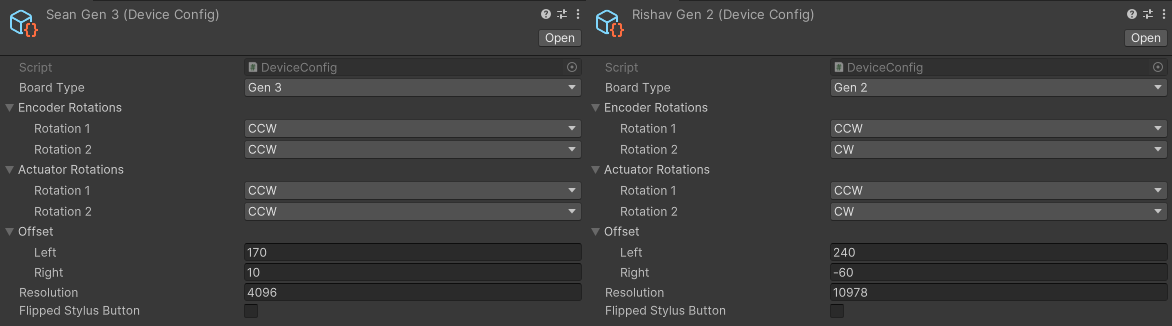
\includegraphics[width = 0.8\textwidth]{images/board-config.png}
    \caption{Different board configurations for the Haply}
    \Description{Different board configurations for the Haply}
    \label{fig:board-config}
\end{figure}

\subsubsection{Utilising Unity's Physics}
The main benefit to utilisng Unity was to leverage it's physics engine for automated haptic experiences. The process of connecting the Haply to Unity physics has been described in detail in \ref{subsec:virtual-coupling}. There are minor nuances in  the implementation itself, specific to Unity. These include making sure the physics engine is running at a higher framerate than normal since the physics is separated from the graphics, enabling continuous collisions for a smoother experience, and interpolating all collisions. While these changes require higher compute, our current application runs at 500+ frames per second, and generally improve the experience without any significant detrmiment to the performanc of the program.

\subsection{Zooming}
In order to allow the designer and user to explore the world at different scales, we incorporate the ability to zoom in and out of the world. From a design perspective, we wished to convey the sense of scale of the world. This was achieved by letting the user explore the ground and the side surfaces of objects in the world when small, and allowing the end effector to "climb" on top of clumps of objects when large, thereby providing force feedback on the basis of the top surface geometry of the objects. 

Implementing this practically was rather trivial, since we had worked extensively on abstracting the texture and object force feedback information. By changing the scale of the representation and moving the camera a proportional amount to said scale, the correct forces and texture data was automatically conveyed. Note that the relationship between the camera's movement and the scaling of the end effector is a cubic one. This is in order to maintain an approximte size of the end effector on screen, such that it gives the appearance of the world growing and shrinking around the designer or the user.

\subsection{Painting}
The incorporation of painting capabilities for objects and textures within a terrain editor is imperative for a multitude of reasons. 
Firstly, such functionality facilitates the creation of intricate and visually captivating landscapes by allowing users to precisely apply diverse textures and objects onto terrain surfaces, thereby enhancing realism and aesthetic appeal. 
More specifically, with the ability to add their own textures and objects, this feature enables users to customize their environments with precision, enabling the realization their artistic visions. 

\begin{figure}[htbp]
    \centering
    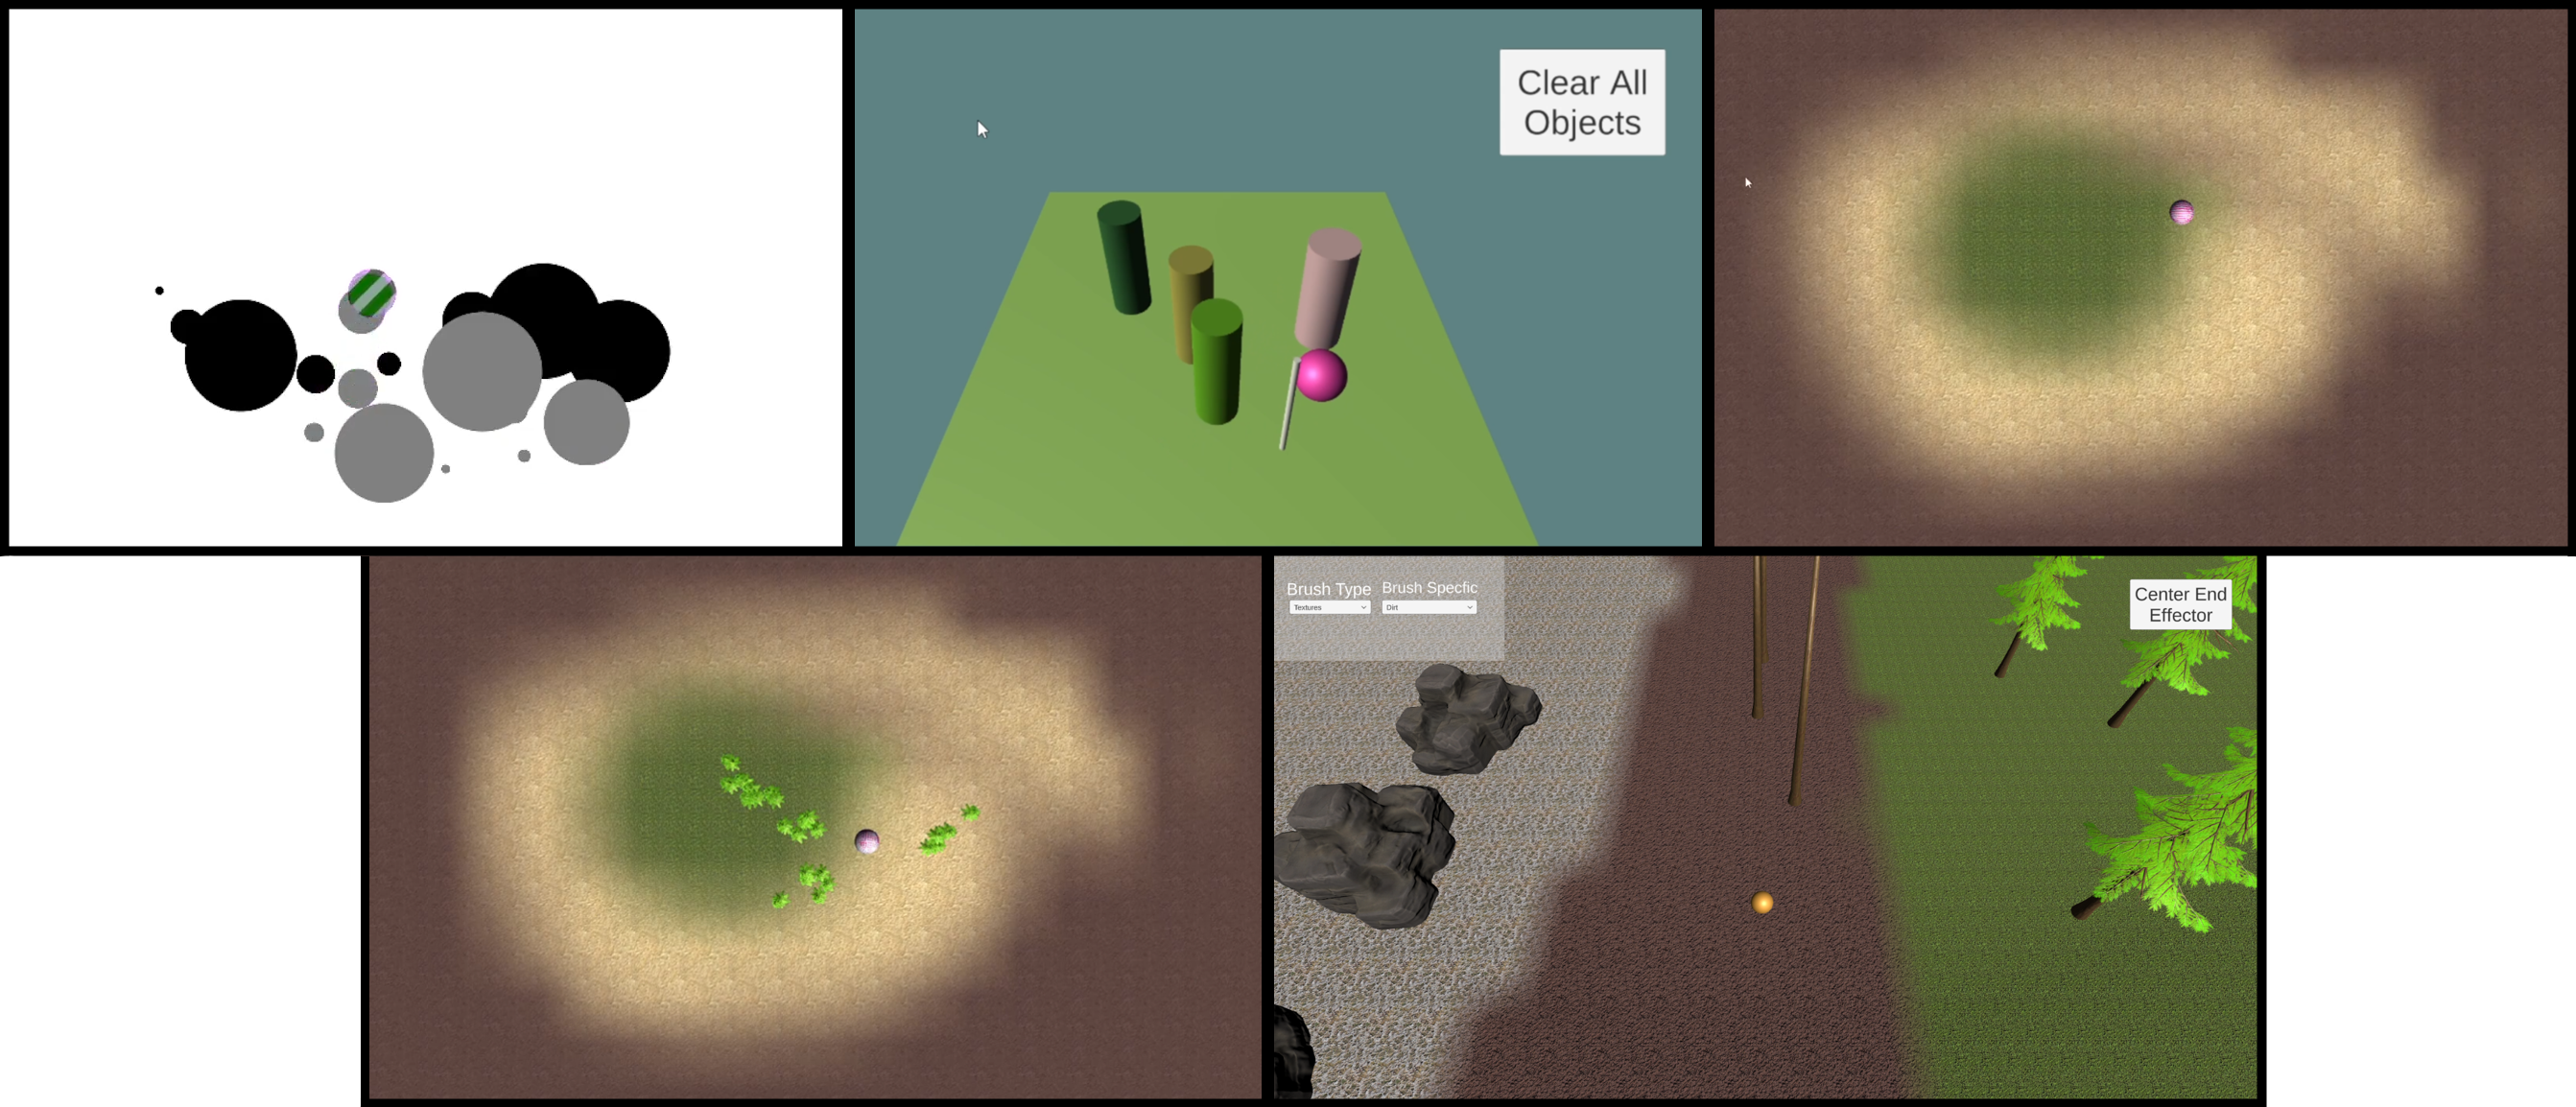
\includegraphics[width=0.8\textwidth]{images/timeline.png} 
    \caption{Representation of the evolution of the prototypes throughout the development of the project
    (1) shows screenshot of the first prototype made to validate our first iteration
    (2) reprensents a screenshot of the first prototype after some code clean up and transfered to 3D space
    (3) displays a screenshot of the texture painting working on Unity's terrain game object
    (4) illustrates painting objects on the the terrain previously textured
    (5) is a capture of the final version which can be seen in Fig. \ref{fig:terrain-painting}}
    \Description{Representation of the evolution of the prototypes throughout the development of the project}
    \label{fig:evolution-painting}
\end{figure}

In line with the comprehensive nature of this project, the process of painting underwent multiple iterations of prototypes throughout the development phase. 
In the forthcoming discussion, we shall examine each prototype and elucidate the insights gleaned from them. 
The creation of our initial prototype, referred to as "the sprinkler," transpired towards the end of the first iteration. 
Its primary objective is to validate the efficacy of the PD controller implementation and the integration of Haply's API for the third iteration of Haply's 2DIY. 
This prototype functioned as a testament to the feasibility of dynamically generating objects during runtime and eliciting force-feedback from interactions between the end-effector and these aforementioned objects.
As illustrated in Figure \ref{fig:texture-rendering}. (1), the sprinkler is placing gray circles as long as we were pressing the stylus button or the spacebar\footnote{the spacebar is used as backup throughout the project if the stylus button doesn't work for diverse reasons}.
These gray circles serve as visual indicators devoid of collision detection, providing a prelude to the subsequent placement of black circles, complete with colliders, upon the eventual release of the stylus button or the spacebar key.


Just after finishing the transition from 2D to 3D, we repurposed the code of "the sprinkler" to be usable in 3D space since it is a quick way to, once again, determine wether or not everything is working as intended.
We are reusing the same logic behind the placement of object as it has proven effective for the first prototype.
In the second image of Figure \ref{fig:texture-rendering}., we can see that the scene is now in 3D and what was previously circles are now cylinders with random colors.
The force-feedback is kept the same, if we move the End-Effector into a cylinder, we will be pushed out as if it is a wall.
We concluded from this prototype that handling the object placement using a similar script is aligned with our goals for object placement, especially since it is easy to use and learn how to use it, thanks to the stylus affordance. 

The subsequent prototype aims to enhance information retention across multiple executions. 
Our approach pivots towards leveraging Unity's terrain game object, which inherently retains terrain deformation, applied textures, and placed objects. 
This strategic alignment enables seamless integration with Unity's terrain editing system, obviating the need for extensive bespoke implementation. 
This not only yields temporal efficiencies but also enhances usability, capitalizing on user familiarity with the platform. 
Our primary focus lies on object and texture painting, thereby excluding terrain elevation adjustments. 

In the prototype corresponding to Figure \ref{fig:texture-rendering}. (3), we introduced the capability to paint textures via mouse input. 
Employing mouse-based prototyping expedites debugging processes, preempting potential issues arising from haptic interfaces. 
This prototype proved its importance in facilitating rapid parameter experimentation, refining aspects such as brush radius, fall-off characteristics, and curve adjustments to ensure smoother edge rendering during texture painting.
From this prototype as a base, we implemented object creation for terrain and object deletion, still utilizing the mouse as an input.
Similarly, it permitted us experiment with different parameters to find what feels best, user experience-wise. 
The results are displayed in Figure \ref{fig:texture-rendering}. (4).

Subsequently, the amalgamation of prototypes culminated in a singular definitive outcome, as depicted in Figure \ref{fig:texture-rendering}. (5).
Firstly, we transitioned the painting process to be contingent upon the positional data of the end-effector representation. 
Secondly, we repurposed the coroutine mechanism utilized for object painting from the second prototype, integrating it seamlessly with newly devised functionalities for object and texture painting, as well as object erasure. 
Lastly, we devised a concise user interface, affording runtime modifications of tools and their respective painting attributes.

\subsection{Texture}
Our initial approach to texture rendering involved firing a raycast to detect the material underneath the end effector. This would then return the corresponding texture information, and the 3x3 window of pixels specifically underneath the end effector representation. Using this we could extrapolate the ideal direction the end effector should be moving. However using raycasts were computationally expensive, and required us to rethink our approach. The texture rendering process in it's current state has been described in detail in \ref{subsec:texture-rendering}, and overall performs better while retaining accuracy in its representation.
